% !TEX root = macfp_2017_gasphase.tex

\subsection{Case 5: Flame Extinction} \label{sec:flame_extinction}

\begin{figure}
\centering
(a)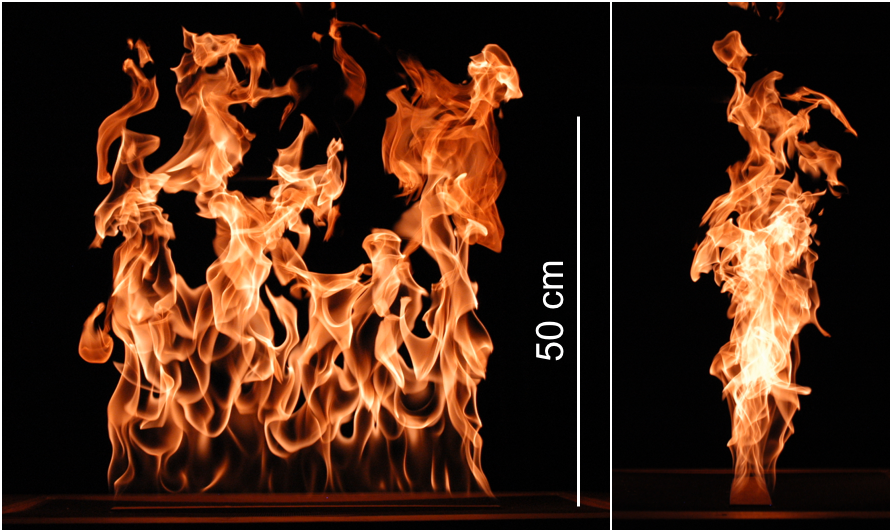
\includegraphics[height=1.3in]{Figures/Case5-Fig1a.png}
(b)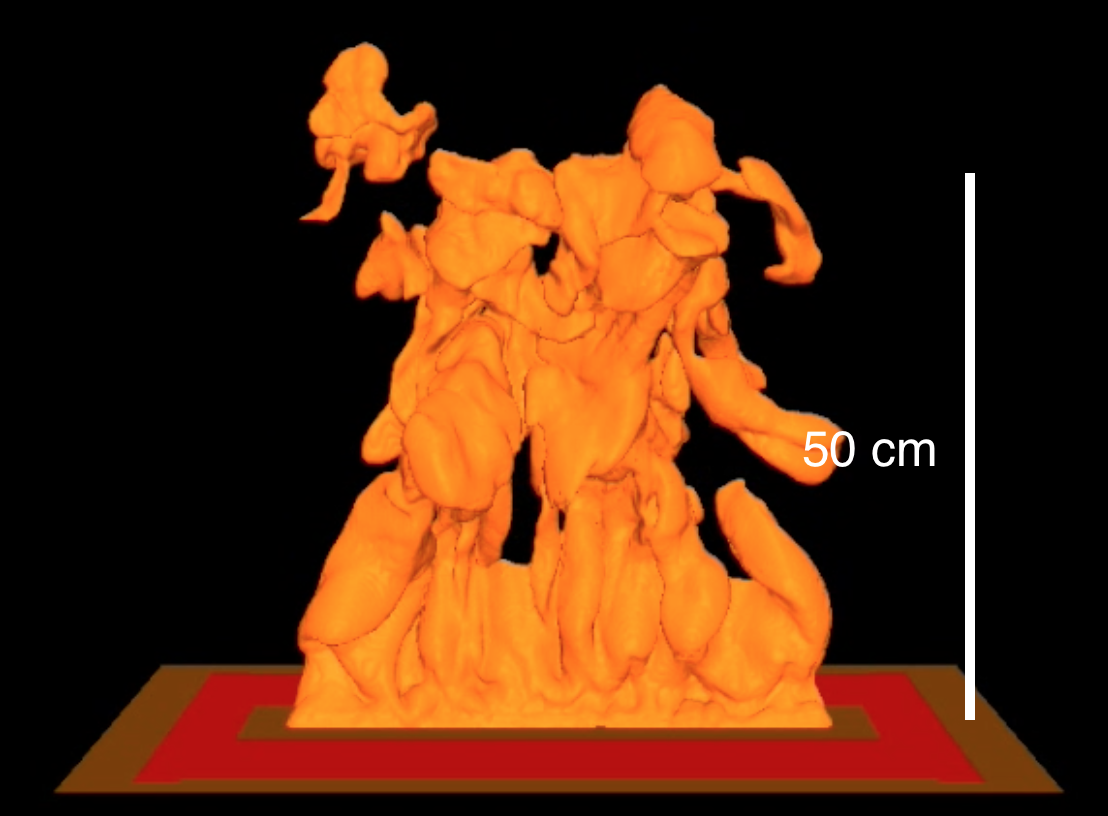
\includegraphics[height=1.3in]{Figures/Case5-Fig1b.png}
(c)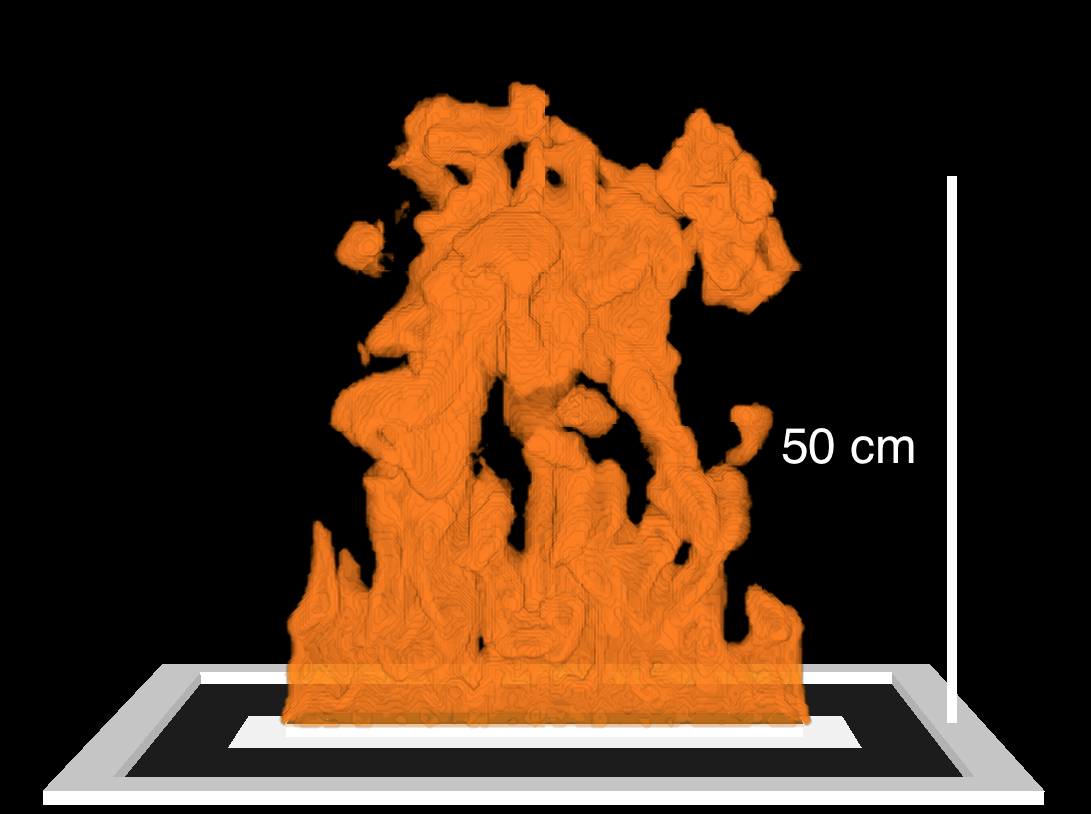
\includegraphics[height=1.3in]{Figures/Case5-Fig1c.png}
\caption{Case 5. Instantaneous snapshot of the methane-air flame in the UMD turbulent line flame experiment: (a) experiment (both front and side view); (b) FireFOAM simulation (front view); (c) FDS simulation (front view). In all figures, the vertical white line indicates 50~cm elevation.}
\label{fig:Case5-Fig1}
\end{figure}

\subsubsection{Experiment}

The flame extinction experiment selected for the first MaCFP workshop is a canonical line-fire configuration with controlled co-flow studied at the University of Maryland (UMD)~\cite{Case5_EXP_1,Case5_EXP_2,Case5_EXP_3}. The UMD turbulent line burner facility allows the study of a buoyancy-driven, turbulent diffusion flame exposed to environments of decreasing oxygen strength, down to the oxygen extinction limit, and thereby provides fundamental information relevant to fire suppression due to under-ventilation or due to the activation of an inert gas system. The facility comprises a sand-filled, stainless-steel fuel port, slot burner, 5-cm-wide and 50-cm-long. Controlled suppression of the flame is achieved via the introduction of nitrogen gas into the co-flowing oxidizer stream.

Both methane and propane fuels were utilized. Assuming complete combustion, the total heat-release rate was 50~kW for both fuels (the flame was approximately 0.5~m-high). The quantitative metric of suppression is the global combustion efficiency, $\eta$, reported as a function of the coflow oxygen strength and measured using oxygen consumption and carbon dioxide generation calorimetry~\cite{Case5_EXP_3}. The mole fraction of oxygen, $X_{\text{O}_2}$, was measured using a paramagnetic oxygen analyzer via a probe located inside the oxidizer port. Infrared radiative emissions were measured using a water-cooled Schmidt-Boelter heat-flux transducer; heat flux data were then converted to global radiative loss fractions using a weighted multipoint radiation source model~\cite{Case5_EXP_2}. Visible flame height was measured using a video camera. A limited set of temperature measurements is also available for methane fuel and $X_{\text{O}_2} = 18 \%$.

\begin{figure}
\centering
(a)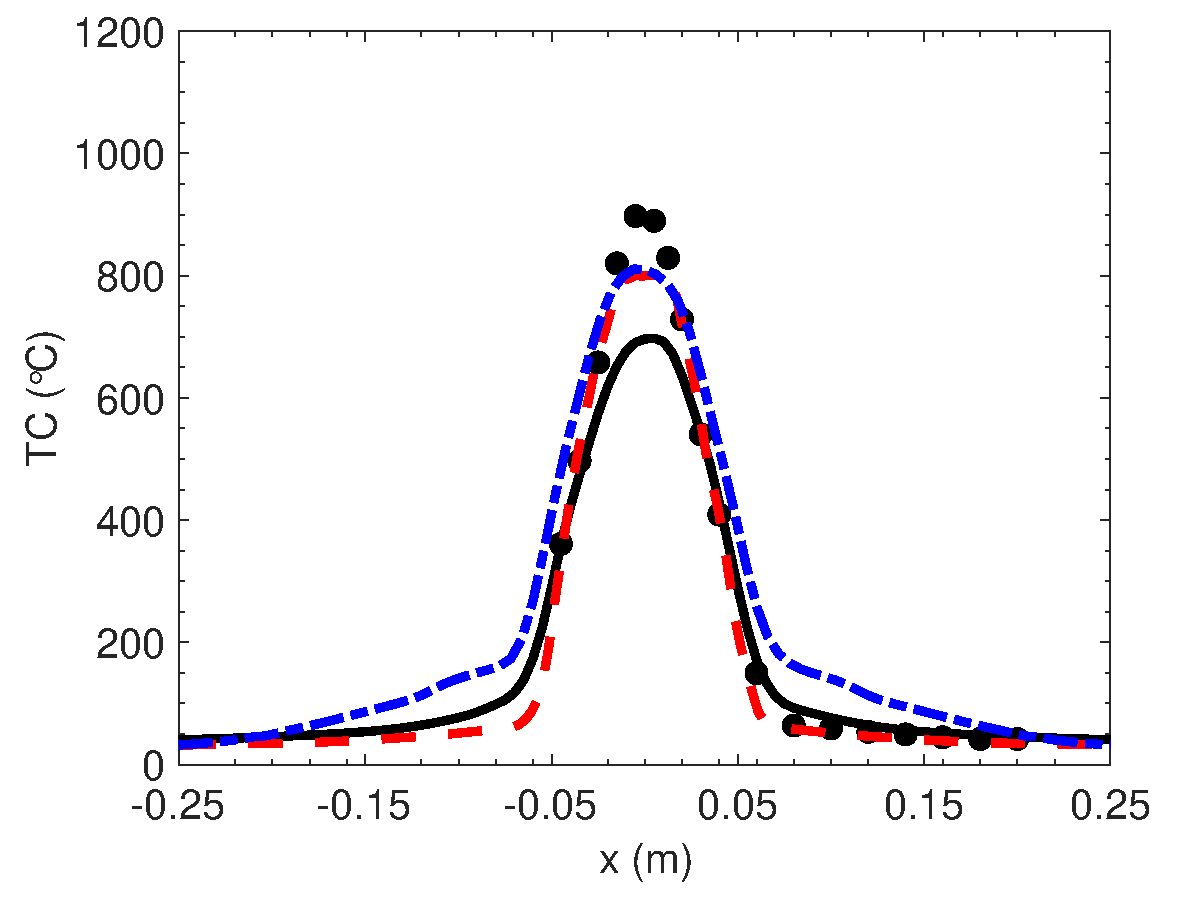
\includegraphics[height=2.2in]{Figures/Case5-Fig2a.pdf}
(b)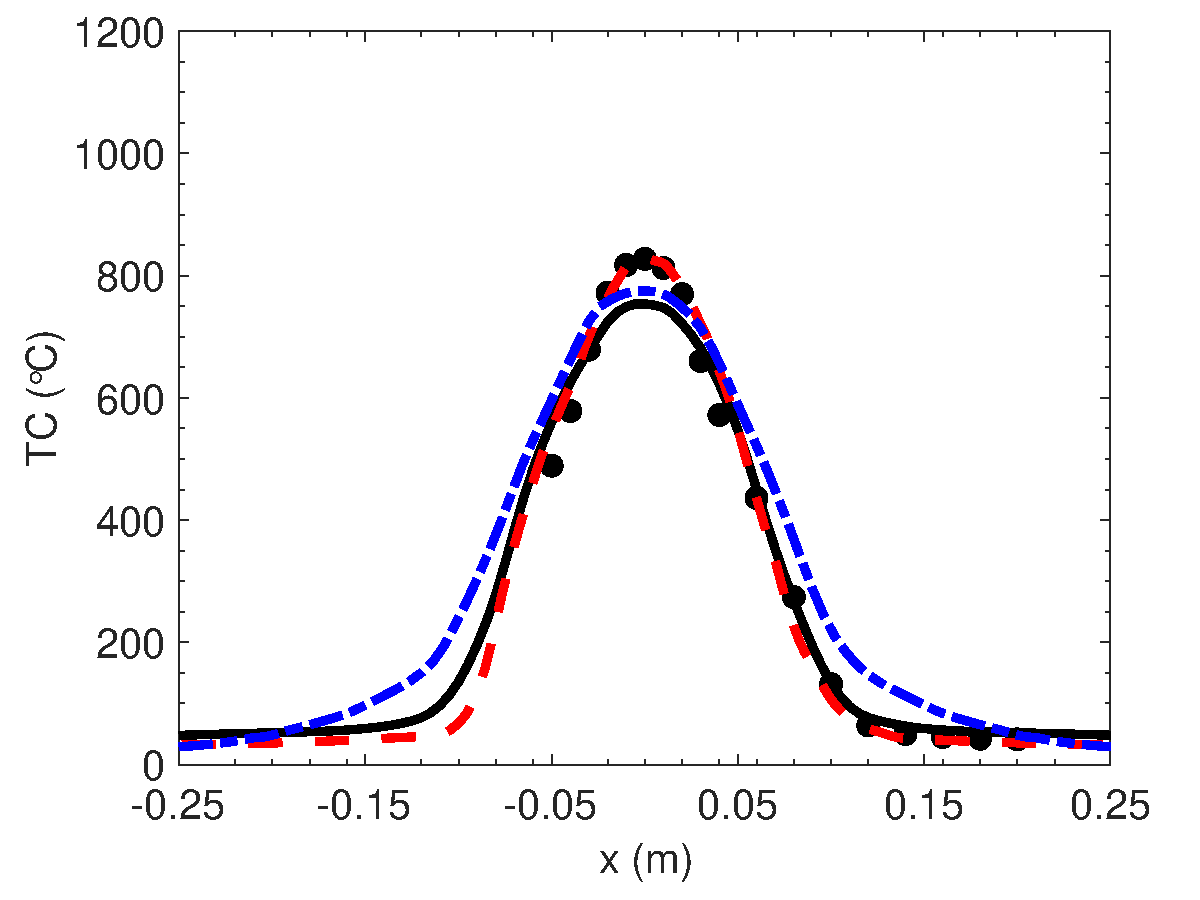
\includegraphics[height=2.2in]{Figures/Case5-Fig2b.pdf}
\caption{Case 5. Cross-flame variations of mean thermocouple temperature at: (a) $z = 0.125$ m; (b) $z = 0.25$ m. Comparison between experimental data (black circles) and numerical results from FM Global (black solid line), NIST (red dashed line), UMD (blue dash-dotted line). Case of a methane flame with $X_{O_2} = 18\%$. 
\label{fig:Case5-Fig2}}
\end{figure}

\subsubsection{Simulations}

Three groups submitted computational results for Case 5: FM Global~\cite{Case5_SIM_FMG}, NIST~\cite{Case5_SIM_NIST} and UMD~\cite{Case5_SIM_UMD}. FM Global and UMD used a shared development version of FireFOAM (FireFOAM-dev)~\cite{FireFOAM}; NIST used an official release of FDS (version 6.5.3)~\cite{FDS}.

As discussed in section~\ref{sec:CGD}, the main challenge found in the design of a computational grid for LES simulations of the UMD turbulent line flame experiment is to provide suitable grid resolution to capture the controlling length scale of the burner, $i.e.$ the burner width (5~cm). This requires millimeter-scale resolution. The computational groups responded to this challenge in a similar way and adopted a resolution of 5-mm (FM Global), 3.125-mm (NIST) and 4.2~mm (UMD) in the flame region.

Additional differences in the numerical treatment of the line flame experiment include differences in the choice of physical models (see section~\ref{sec:PM} for details on baseline choices). FM Global and UMD used the baseline configuration of FireFOAM except for the addition of a flame extinction model based on the concept of a critical Damk\"ohler number for premixed eddies~\cite{Dorofeev:2016} (FM Global) or the concept of a critical Damk\"ohler number for diffusion flames~\cite{Vilfayeau:2016} (UMD); the values of the global radiative loss fraction were prescribed using the measured values~\cite{Case5_EXP_2}; in the solution of the RTE, the discretization of angular space used 16 angles. NIST used the baseline configuration of FDS except for the addition of a flame extinction model based on the concept of a critical flame temperature~\cite{Vaari:2011,White:2017}; in the solution of the RTE, the discretization of angular space used 700 angles (the large number of angles is due to the fact that the NIST simulation included the heat flux gauge located at 1-m distance from the flame and was motivated by the desire to avoid any potential ray effect). 

\begin{figure}
\centering
(a)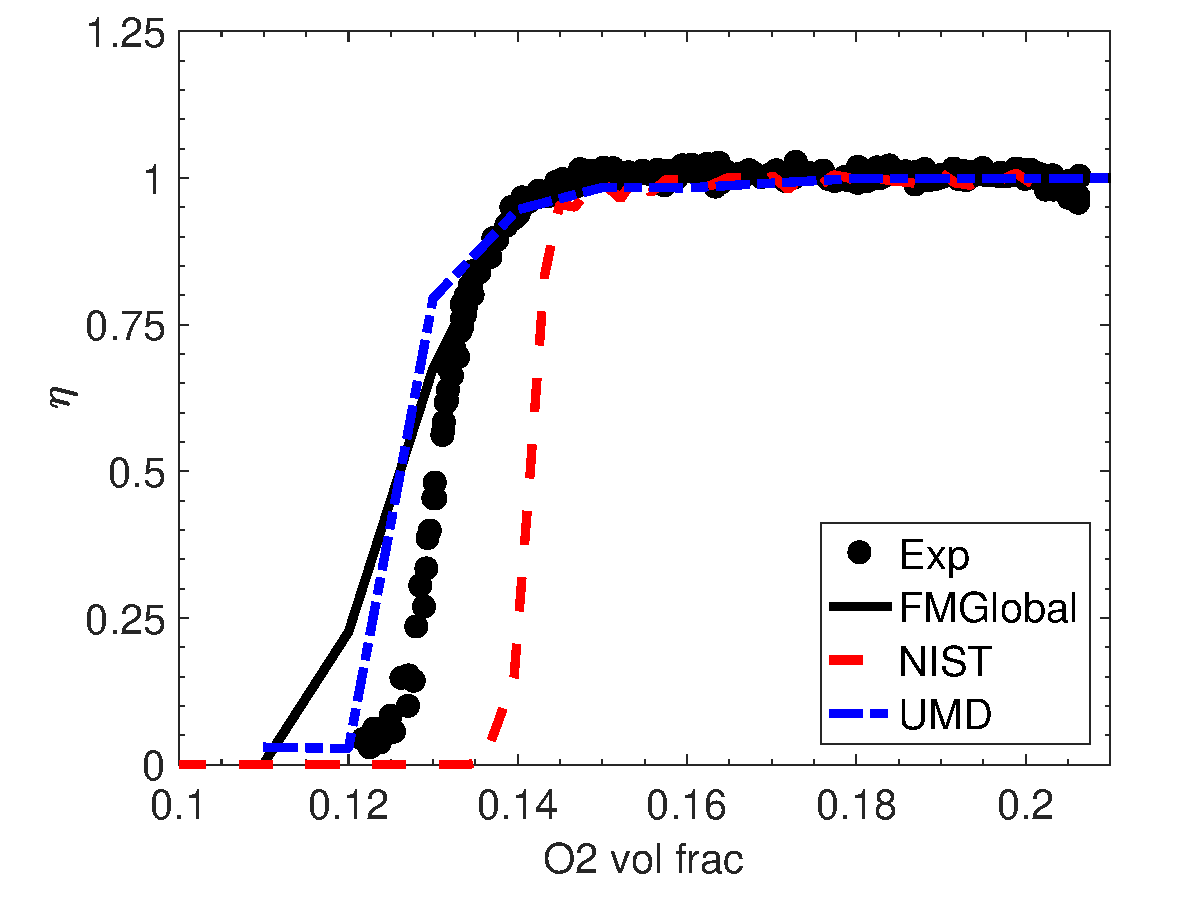
\includegraphics[height=2.2in]{Figures/Case5-Fig3a.pdf}
(b)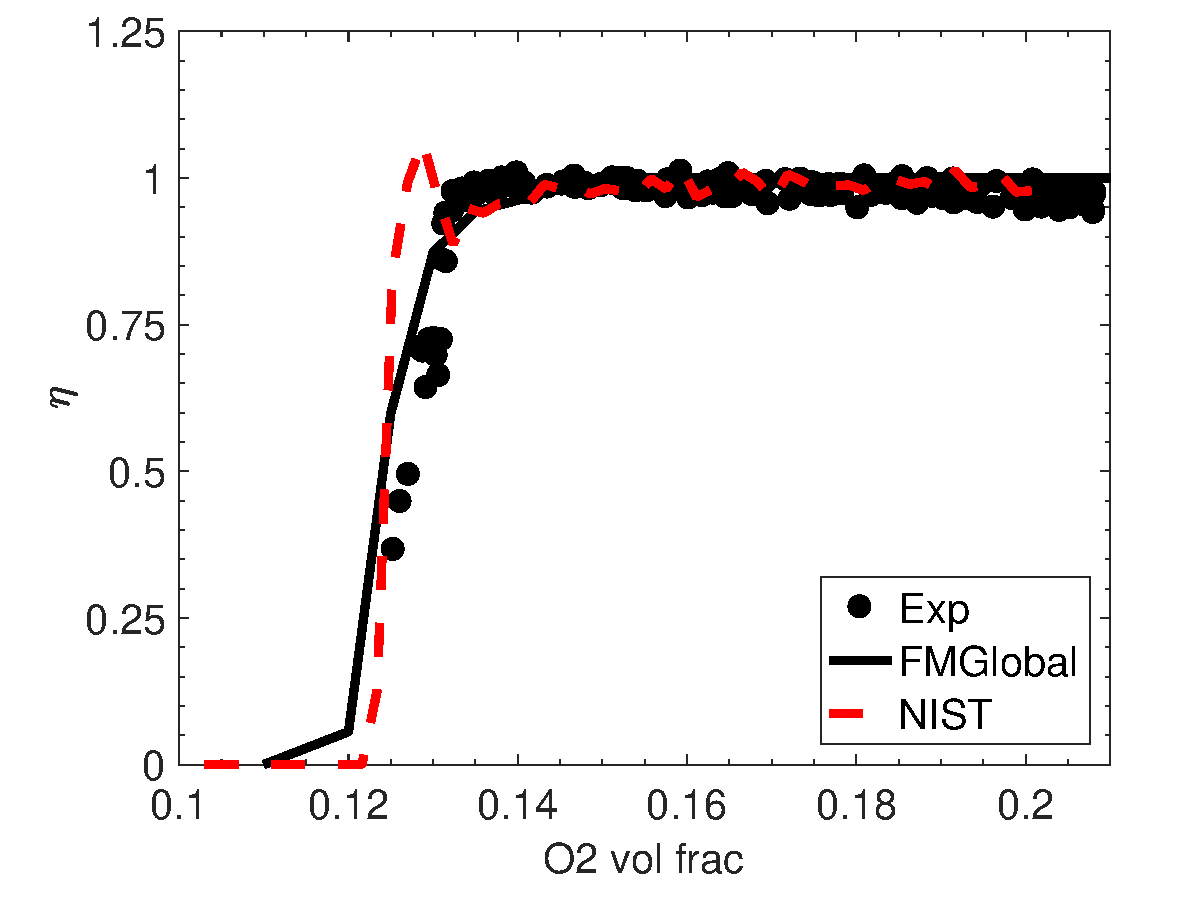
\includegraphics[height=2.2in]{Figures/Case5-Fig3b.pdf}
\caption{Case 5. Variations of the global combustion efficiency with the coflow oxygen mole fraction. (a) methane flame; (b) propane flame. See caption of Fig.~\ref{fig:Case5-Fig2}.}
\label{fig:Case5-Fig3}
\end{figure}

\subsubsection{Summary}

All simulations seem to reproduce the overall structure of the turbulent flame (see Fig.~\ref{fig:Case5-Fig1}.). Figure~\ref{fig:Case5-Fig2} presents comparisons between measured and simulated thermocouple temperatures performed at quarter-flame height and at mid-flame height (note that in these comparisons, all simulations use a thermocouple model). Figure~\ref{fig:Case5-Fig2} suggests that the level of agreement between experimental data and numerical results is encouraging; discrepancies are however observed, especially at quarter-flame height, and those may be attributed to inaccuracies in the combustion model, in the thermal radiation model, or in the coupling of these models.

Figure~\ref{fig:Case5-Fig3} presents comparisons between measured and simulated combustion efficiencies as a function of the coflow oxygen strength,  for both methane and propane flames. All simulations correctly reproduce the binary nature of the flame response: the combustion efficiency remains close to 1 for $X_{\text{O}_2}$ above the extinction limit and abruptly decreases to 0 at this limit ($i.e.$ for $X_{O_2} \approx$ 12-14 \%). The exact value of the oxygen extinction limit is predicted within $\pm$ 10-20\%. While these results are encouraging, it is worth emphasizing that the flame extinction models are complex (they in fact rely on a description of both extinction and re-ignition phenomena~\cite{Dorofeev:2016,Vilfayeau:2016,White:2017}) and that the models used in the FM Global, NIST and UMD simulations are based on different representations of the physics. Thus, the UMD turbulent line flame database is not capable of differentiating between the three flame extinction models and therefore does not provide sufficient insight into the underlying physics of flame suppression. Also, as mentioned in section~\ref{sec:CGD}, it is important to recognize that the FM Global and UMD flame extinction models (and to a lesser extent the NIST flame extinction model) were originally tuned against data obtained from the same UMD experiment. Therefore, the simulations should be interpreted as \emph{calibration} tests rather than validation tests.

Note that the UMD turbulent line flame database has been recently enhanced with new micro-thermocouple measurements and has also been extended to the case of flame suppression by a water mist~\cite{Case5_EXP_1}. These new developments should be incorporated into MaCFP. The addition of micro-thermocouple measurements will provide much needed data to characterize the details of the flame structure (and will provide both first- and second-order statistics). More information on flow velocity as well as on gas and soot radiation will also be needed in order to unravel the respective effects of combustion and thermal radiation.











